\section{Synthetic database creation}\label{sec:benchmark:database}
Synthetic databases are critical to running a customisable and repeatable
benchmark. Those who wish to benchmark a database can use custom synthetic
databases in order to specify a large amount of unknowns in the data of the
benchmarks run. Examples of such parameters range from both the size of the
database as a whole to on a tuple level by carefully choosing attribute domains.
Attribute domains can also help give a heuristic control to resource load while
processing queries by determining how difficult it is to computer an answer (for
instance using the equality of strings). Furthermore, when designed correctly synthetic
databases can provide a readable method to easily specify wanted properties of
queries via explicit and easy to calculate selectivity factors in selections and
joins. More information on database benchmark design can be found in
\fref{sec:background:benchmarkbestpractices}.

\paragraph{} In order to have a customisable synthetic benchmark for the
project, we created a collection of python modules to easily configure and
export different databases. We chose to implement this as an extensible set of
classes to represent different cell domains which then can be configured,
specified and passed to objects representing larger structures of the database
and handle generation for each of their responsibilities. This section is a
walk through the ensuing python modules and their internal relationships.

\begin{wrapfigure}{R}{0.4\textwidth}
    \centering
    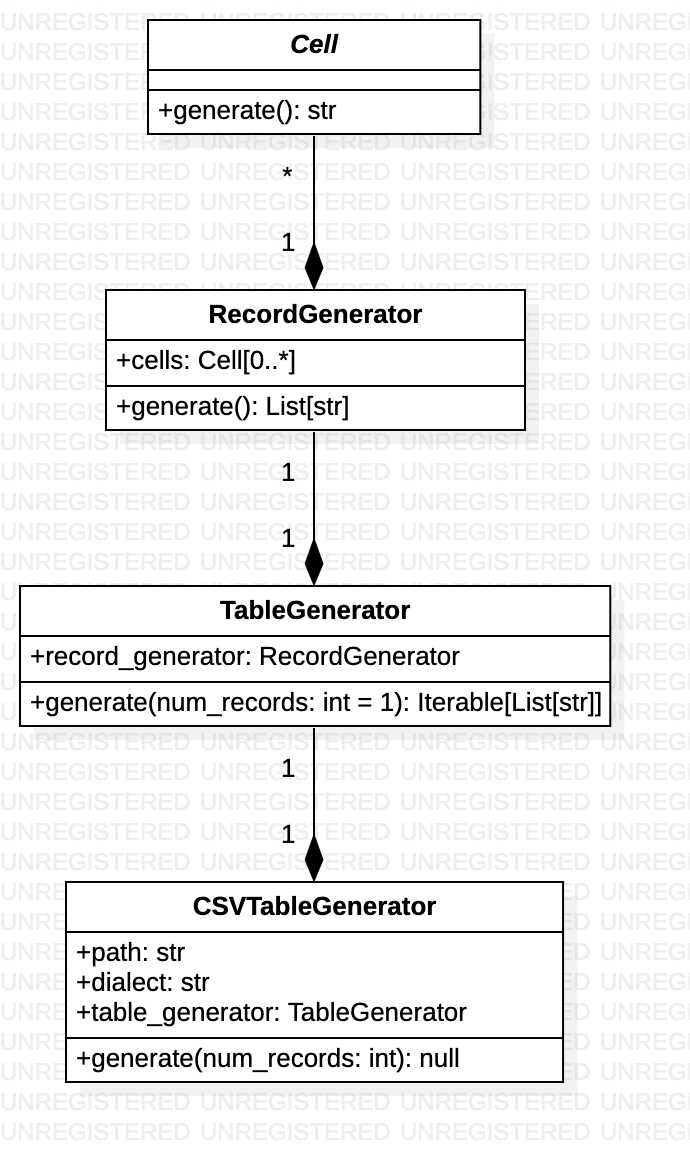
\includegraphics[width=0.4\textwidth]{project/benchmark/database_generation_class_diagram}
    \caption{UML class diagram showing the modules used for synthetic database
    creation.}
    \label{fig:project:benchmark:creation-class-diagram}
\end{wrapfigure}

\paragraph{Overview} This section describes the overall structure of the
solution, a class-diagram to aid the explanation can be found in
\fref{fig:project:benchmark:creation-class-diagram}.
We start with a list of objects extending the \lstinline{Cell}
abstract class. We pass this list to a \lstinline{RecordGenerator} object, which
then can be given to a \lstinline{TableGenerator} object to generate the
database. Finally the database generator can be given to an object, such as the
implemented \lstinline{CSVTableGenerator} to create the
specified output. The advantages of this approach is the ability to easily
configure a handful of properties of the output database by varying just the list of cells.
Cells can be easily manipulated given they conform to the \lstinline{Cell} API
and so their basic capabilities cover a large amount of behaviour and
compositions.
